\documentclass{article}
\usepackage{bookmark}
\usepackage{hyperref}
\usepackage{graphicx}
\usepackage{textcomp}


\title{The Online Movie Catalog}
\author{Cavagnino Matteo}


\begin{document}
\maketitle

\section{Richiesta e requisiti}
Il progetto sviluppato \emph{The online movie catalog} è l'applicazione web con lo scopo di rappresentare un portale in grado di permettere a utenti venditori di creare il proprio
negozio e vendere i loro prodotti e agli utenti clienti di comprarli.
La richiesta è quindi quella di realizzare l'intera applicazione assicurandosi di includere determinati requisiti in modo coerente.

    \subsection{Requisiti dei venditori e dei negozi virtuali}
    La prima categoria di utenti è quella dei venditori, essi devono essere in grado di:
    \begin{itemize}
        \item Registrarsi all'applicazione
        \item Creare il proprio negozio virtuale
        \item Modificare i propri dati
        \item Cancellare il proprio account
        \item Tenere sotto controllo il flusso di vendite
        \item Aggiungere in qualsiasi momento nuovi prodotti al proprio catalogo
        \item Modificare/cancellare i prodotti dal proprio catalogo
    \end{itemize}

La seconda categoria di utenti è quella dei clienti, essi devono essere in grado di:
    \begin{itemize}
        \item Registrarsi all'applicazione
        \item Modificare i propri dati
        \item Cancellare il proprio account
        \item Acquistare o noleggiare film da un negozio virtuale a scelta
        \item Scegliere se mantenere memorizzate le proprie informazioni relative ai pagamenti
        \item Aggiungere ed eliminare prodotti dal carrello per effettuare acquisti multipli
    \end{itemize}


\section{Login, registrazione e struttura dei dati}
    \subsection{Processo di registrazione}
    La prima fase che un utente deve attraversare è quella relativa alla registrazione del proprio account.
    In tale fase è richiesto a tutti gli utenti di inserire:
        \begin{itemize}
            \item Nome
            \item Cognome
            \item E-mail
            \item Password (e conferma password)
            \item Accettare i termini sulla privacy
        \end{itemize}
    Dopodichè viene richiesto all'utente di selezionare il proprio ruolo tra i due disponibili: cliente e venditore. In base a tale scelta verranno mostrati altri campi che
    richiedono l'attenzione dell'utente.
    Nel caso il ruolo selezionato sia \emph{cliente} verrà mostrata una casella per la preferenza sulla raccolta di dati aggiuntivi da parte dell'applicazione,
    se invece, il ruolo selezionato è \emph{venditore} verranno mostrati i seguenti campi da compilare:
        \begin{itemize}
            \item Nome negozio
            \item Numero di telefono
            \item Partita iva
            \item Indirizzo (città, cap, via, numero civico)
        \end{itemize}
    Dopo aver compilato tutti i campi necessari l'utente potrà accedere al proprio account.


    \subsection{Gestione dati in fase di registrazione}
    Tutti i dati vengono memorizzati tramite l'uso di \emph{cookie, local storage e session storage} sotto forma di documenti JSON.
    Per quanto riguarda le informazioni relative agli utenti vengono specificati all'interno del documento tutti i campi in comune (come nome e cognome) più un campo \emph{Extra} in cui vengono specificati tutti i campi non in comune (come nome negozio e servizi personalizzati).
    Il vantaggio di questa organizzazione è che i documenti rimangono semplici da interpretare dallo sviluppatore e le query vengono semplificate.
    Per la gestione di molte delle funzioni dell'applicazione sono state usate come supporto le liste offerte dalla WEBAPI \href{https://developers.themoviedb.org/3/getting-started/introduction}{TheMovieDB}.
    \paragraph{Dati del cliente}
    In fase di registrazione da parte di un utente \emph{cliente} le informazioni compilate nel form vengono memorizzate nel \emph{local storage} del browser seguendo la struttura in \emph{Figure 1}
    Ovviamente non tutte le informazioni saranno subito presenti al momento della registrazione, tale fatto verrà discusso nelle prossime sezioni.
    Al momento della registrazione, sulla WEBAPI verrà creata una lista che conterrà tutti i titoli acquisiti dall'utente.
    \begin{figure}
        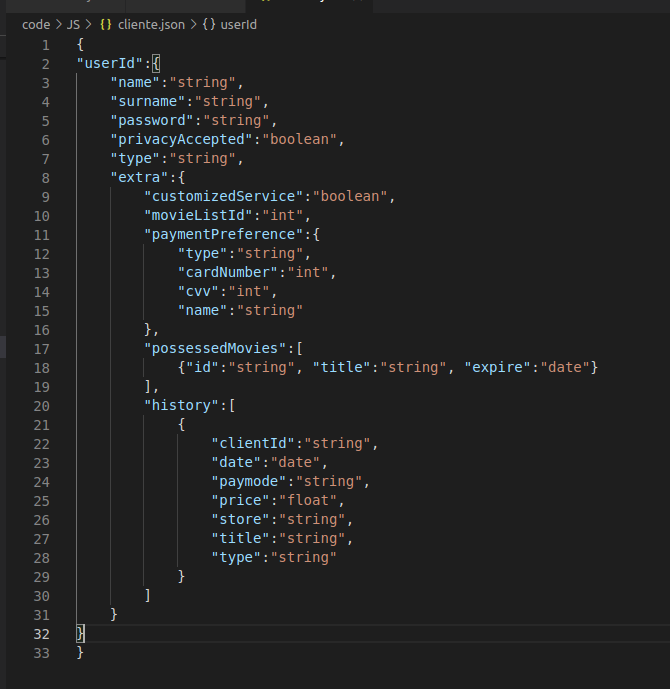
\includegraphics[width=\textwidth,height=\textheight,keepaspectratio] {img/cliente.png} 
        \caption{Struttura dati cliente}
    \end{figure}
    \begin{figure}
        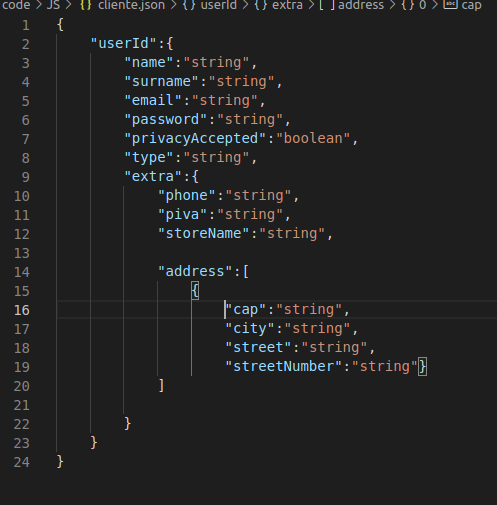
\includegraphics[width=\textwidth,height=\textheight,keepaspectratio] {img/vendor.png} 
        \caption{Struttura dati venditore}
    \end{figure}


    \paragraph{Dati del venditore}
    Per quanto riguarda l'organizzazione dei dati dell'utente \emph{venditore} essa è molto simile a quella del \emph{cliente} (v. \emph{Figure 2}), la differenza è
    che per il venditore verrà creata una lista sulla WEBAPI contenente tutti i prodotti in vendita e un'ulteriore documento JSON contenente le informazioni relative al negozio (quest'ultima usa come chiave il nome stesso del negozio, il quale e' univoco):
    \begin{itemize}
        \item ID lista WEBAPI
        \item lista delle vendite (con relative informazioni)
        \item lista dei prodotti in vendita
    \end{itemize}

    Inoltre per facilitare l'accesso a tutti i nomi dei negozi è stato creato un documento (sempre memorizzato nel local storage) contenente una semplice lista dei nomi dei negozi registrati;
    in fase di registrazione di un venditore il suo negozio verrà quindi inserito in tale lista.
    L'unica scelta implementativa effettuata in fase di registrazione è quella di non permettere a due utenti di registrarsi con la stessa email (dato che lo userId viene generato con un \emph{hash} usando per l'appunto l'email).

    \subsection{Gestione dei dati in fase di login}
    Per verificare l'identità di un utente in fase di login, viene calcolato un \emph{hash} utilizzando la email inserita, cercato l'account nel local storage con l'id ricavato
    ed infine viene controllato che la password sia corretta.
    \paragraph{Sessioni}
    Al momento del login, viene aggiunta al cookie una chiave \emph{session} che ha come valore l'id dell'utente e come scadenza 5 minuti se l'utente si è appena registrato o se 
    ha loggato senza specificare la casella \emph{Ricordami}, se invece l'utente ha specificato tale checkbox la scadenza diventa nulla (ovvero viene imposto un valore molto elevato).

    Viene quindi creata una sessione per l'utente e memorizzata anch'essa nel local storage sotto forma di documento JSON.
    In tale documento viene memorizzata la scadenza della sessione e l'id dell'utente (inoltre per i clienti tale sessione contiene anche il carrello con i prodotti).

    Le sessioni vengono eliminate nel momento in cui scadono e nel momento in cui l'utente effettua il logout, vengono inoltre sovrascritte se un altro utente effettua il login.

\section{Funzionalità venditore}
    \subsection{Aggiunta prodotti al proprio catalogo}
    La pagina default per l'utente venditore e' quella per l'aggiunta di prodotti al proprio catalogo.
    In tale pagina l'utente può selezionare molteplici titoli e aggiungerli tutti insieme alla propria lista di prodotti,
    le informazioni riguardanti i film aggiunti verranno aggiunte al documento JSON nel local storage relativo al negozio e alla lista sulla WEBAPI.
    Su questa pagina (e in seguito su ogni pagina relativa a liste di film) è abilitata la funzione di ricerca, tale funzione, presente solo in questa pagina, fa uso di uno dei metodi
    messi a disposizione dalla WEBAPI per effettuare una ricerca efficiente in tutto il database.
    Inoltre,
    per ogni film e' possibile cliccare un bottone che aprirà una pagina con maggiori informazioni sul film.
    \subsection{Il catalogo}
    La pagina del catalogo mostra tutti i film messi in vendita dall'utente, anche in questa pagina è abilitata la funzione di ricerca ma qui quest'ultima ha un funzionamento differente dato che 
    la WEBAPI non fornisce un metodo per la ricerca all'interno delle liste.
    Per effettuare la ricerca viene creata in fase di setup dell'applicazione una lista apposita per questa funzione sulla WEBAPI, la ricerca viene effettuata sulla lista di film
    memorizzata nel documento relativo al negozio nel localstorage, i film risultanti vengono aggiunti alla lista sulla WEBAPI e infine con una sola operazione di \emph{GET} vengono prelevati dettagli e locandine di tutti i film.

    \subsection{Cronologia vendite}
    In questa pagina vengono elencate tutte le vendite effettuate con successo, le informazioni mostrate sono:
    \begin{itemize}
        \item Titolo del film
        \item Metodo di pagamento
        \item Tipo di transazione (acquisto o noleggio)
        \item Importo
        \item Id acquirente
        \item Data
    \end{itemize}
    Tali informazioni vengono prelevate dal documento JSON relativo al negozio.

\section{Funzionalità Cliente}

    \subsection{Navigazione negozi}
    La prima pagina in cui il cliente viene portato è la pagina relativa alla scelta del negozio da visitare, 
    in questa pagina è presente un elenco con tutti i negozi disponibili.
    In tale elenco sono fornite le seguenti informazioni per ogni negozio:
    \begin{itemize}
        \item Nome del negozio
        \item Numero di film in vendita
        \item Media delle recensioni di tutti i film
    \end{itemize}
    Cliccando su uno dei negozi l'utente verrà condotto alla pagina del negozio selezionato.
    In tale pagina è presente la lista delle locandine dei film offerti, sui film già in possesso dall'utente è presente
    un piccolo badge che li indica.
    Cliccando su un film di cui non si è in possesso verrà mostrata la pagina del film selezionato con le relative informazioni complete (titolo, generi, descrizione)
    assieme ad una lista orizzontale contenente tutti gli attori partecipanti e assieme ai bottoni necessari per acquistare/noleggiare il film o aggiungerlo al carrello.
    Se si sceglie di acquistare o noleggiare un film senza passare dal carrello, verrà mostrata direttamente la pagina del pagamento.

    \subsection{Pagamenti}
    Riguardo ai pagamenti, se l'utente ha specificato in fase di registrazione che vuole avere dei servizi aggiuntivi,
    dopo il primo pagamento verranno salvate tutte le informazioni necessarie per rendere il pagamento successivo istantaneo.
    Tali informazioni (relative per esempio alla carta di credito) sono memorizzate nel local storage nel documento relativo all'utente.
    Le opzioni disponibili per il pagamento sono tra carta di credito e PayPal\textregistered, per la carta di credito tutti i controlli affinchè le
    informazioni siano plausibili sono effettuati.
    Nel momento in cui un utente acquista o noleggia un film, questo viene aggiunto alla lista di film posseduti sia nel local storage sia sulla WEBAPI,
    inoltre, la transazione viene memorizzata sia per il cliente sia per il negozio.

    \subsection{Lista dei film posseduti}
    In questa pagina vengono visualizzati i film posseduti dal cliente, tali film vengono prelevati con una singola operazione di \emph{GET} dalla lista personale sulla WEBAPI.
    Se un film è stato noleggiato, sarà presente un piccolo badge che segnala il tempo rimanente (si parte da un totale di 72 ore per il noleggio), allo scadere del quale
    il film verrà automaticamente rimosso sia dal local storage sia dalla WEBAPI.

    \subsection{Carrello del cliente}
    Nella pagina del carrello è presente una lista con tutti i prodotti aggiunti al carrello dall'utente, per ogni prodotto sono presenti le seguenti informazioni:
    \begin{itemize}
        \item Titolo del film 
        \item Media recensioni
        \item Tipo di transazione (acquisto o noleggio)
        \item Prezzo
    \end{itemize}
    All'interno del carrello è possibile scegliere per ogni prodotto se eliminarlo oppure se vederne ulteriori dettagli cliccando sul titolo.
    Sotto la lista è presente il bottone per procedere all'ordine, se cliccato aprirà la finestra per il pagamento con il totale da pagare per tutti i prodotti nel carrello.

    \subsection{Cronologia degli acquisti}
    
    In questa pagina viene mostrato un elenco con tutti gli 
    acquisti effettuati dall'utente, per ogni riga vengono mostrate le seguenti informazioni:
    \begin{itemize}
        \item Titolo del film
        \item Tipo di transazione (acquisto o noleggio)
        \item Prezzo pagato
        \item Nome del negozio
        \item Data
    \end{itemize}

\section{Pagina account}
    Per ogni tipo di utente la pagina dell'account permette di cambiare tutte le informazioni relative ad esso.
    Se un'informazione viene modificata è possibile cliccare il pulsante per confermare i cambiamenti.
    Qui è inoltre presente un bottone per eliminare l'account.
    Nel caso di un utente venditore, eliminare l'account comporta la cancellazione del negozio associato.

\section{Note aggiuntive}
Il cookie viene controllato ogni volta che l'utente cambia pagina, se la sessione è scaduta viene comunicato e l'utente viene riportato alla
schermata di login.
Nel cookie oltre alla sessione viene anche memorizzato se l'utente ha specificato di voler essere ricordato e il tipo di cliente.
Nel session storage non vengono memorizzate informazioni particolarmente importanti, solo qualche informazione nel caso fosse necessario passarla da una pagina all'altra,
ad esempio, quando si clicca su un film, nel session storage viene memorizzato l'id del film e all'apertura della pagina del film uno script si occuperà di usare tale id per 
effettuare una chiamata REST alla WEBAPI per ottenere le informazioni necessarie.

\end{document}